%% chapter 3 Land use and functional diversity

\section*{Keywords}
Land use; land-use intensity; terrestrial vertebrates; functional diversity; traits.

\section*{Abstract}
Land-use change is the leading driver of global biodiversity loss, thus characterising its impacts on the functional structure of ecological communities is an urgent challenge. Using a database describing vertebrate assemblages in different land uses, I assess how the type and intensity of land use affect the functional diversity of vertebrates globally. I find that human land uses alter local functional structure by driving declines in functional diversity, with the strongest effects in the most disturbed land uses (intensely used urban sites, cropland and pastures), and among amphibians and birds. Both tropical and temperate areas experience important functional losses, which are only partially offset by functional gains. Tropical assemblages are more likely to show decreases in functional diversity that exceed those expected from species loss alone. These results indicate that land-use change non-randomly reshapes the functional structure of vertebrate assemblages, raising concerns about the continuation of ecological processes sustained by vertebrates.

\section{Introduction}
Anthropogenic activities are profoundly transforming global biodiversity. Although multiple pressures act in combination, land-use change currently poses the greatest threat to biodiversity \citep{Maxwell2016, Newbold2015}. However, not all species respond similarly to land-use change. Traits have been found to explain species' sensitivity to land-use change in diverse groups \citep{Newbold2013, Nowakowski2017, Quesnelle2014, Todd2017}. Previous work has also shown that land-use change leads to non-random modification of assemblage trait composition (or functional diversity) \citep{Chapman2018, Colin2018, Flynn2009, LaSorte2018, Newbold2013, Tinoco2018}. Since it is widely acknowledged that biodiversity, and in particular trait diversity, may promote ecosystem functioning and stability, modification to the trait composition of assemblages could have far-reaching and adverse impacts on ecological processes \citep{Hooper2012, Magioli2021, Oliver2015, Tilman1994}.

Terrestrial vertebrates support many processes, ranging from pollination \citep{Ratto2018}, to seed dispersal to the regulation of lower trophic levels \citep{Barber2010, Letnic2012, Salo2010,Zhang2018}. However, we lack a global understanding of how the functional diversity of entire vertebrate assemblages responds to changes in land use. Most previous studies have been conducted at regional or local scales \citep{Davison2021}, but these may not be representative of global patterns. Indeed, recent global syntheses have highlighted how biodiversity responses can differ substantially between regions and across latitudes, with higher sensitivity reported for the tropics \citep{Matuoka2020,Millard2021, Newbold2020}. Another key issue is the taxonomic coverage of past work. Few studies investigating effects of land use on functional diversity have considered several vertebrate classes together, and comparative studies remain rare. Thus, how land-use change affects the functional diversity of local vertebrate assemblages at global scales, and the potential geographical and taxonomic variation in the effects, still largely remains to be explored.

Here, I aim to assess how human land use and land-use intensity affect the functional diversity of vertebrate assemblages, across and within taxonomic classes. Building on recent work \citep{Matuoka2020,Millard2021, Newbold2020}, I investigate differences in response between tropical and temperate regions. We use multiple response metrics to quantify functional diversity. First, functional richness measures the breadth and variety of trait combinations represented in an assemblage \citep{Legras2018}. Second, functional dispersion quantifies how similar species in a given assemblage are in terms of their traits \citep{Laliberte2010}. These metrics can mask important alterations of assemblage composition if functional losses are compensated for by functional gains. To address this, we consider pairwise measures between assemblages, to explore levels of functional loss and functional gain across land uses (Figure 1REF).

%% Figure 1 %%

%%%%%%%%%%%%%%

To this end, I combine (1) the trait data across terrestrial vertebrates collected in Chapter 2 (also published in \citep{Etard2020}), with (2) global records of species occurrence in eight land-use types of differing intensity of use (the PREDICTS database \citep{Hudson2014, Hudson2017}, Figure 1, Table S1). The PREDICTS database is currently the most comprehensive database of sampled species occurrence, and for most records also abundance, across multiple land uses of different use intensity. Using the PREDICTS database allows us to contrast biodiversity metrics among intact land uses (primary-vegetation sites, considered to be the undisturbed reference condition), and all other human land-use types. Specifically, we test the following hypotheses, both across and within taxonomic classes:

\begin{enumerate}
\item I expect decreases in functional diversity in human land uses compared to primary vegetation, caused by contractions of occupied trait space. I expect such effects to be more pronounced where land is used more intensively by humans. This hypothesis builds upon evidence that species with certain traits are more sensitive to land-use disturbance \citep{Newbold2013}, meaning that disturbed land uses will retain only disturbance-tolerant species, more functionally similar to one another. Given the reported higher sensitivity of tropical assemblages to land-use disturbance, I predict that such effects are stronger in the tropics.
\item I hypothesise that decreases in functional diversity in disturbed land uses exceed decreases expected by chance, given local species loss. Thus, I expect disturbed land uses to promote functional under-dispersion. Functional under-dispersion occurs when species within an assemblage are more similar, in term of their traits, than expected by chance \citep{Cadotte2017, Wong2018} -- or, in other words, when functional dispersion is lower than expected given local species richness. I predict that under-dispersion is more likely to occur in the highly disturbed sites, in both temperate and tropical areas. This hypothesis is based on the idea that species are being removed non-randomly from sensitive areas of the trait space, and increasingly so with higher disturbance level.
\item Finally, I expect decreases in functional diversity in human land uses to be driven by high functional loss, whereby species are being removed from previously occupied areas of the trait space; I expect no functional gain. This hypothesis is based on the idea that the functional trait space in undisturbed land uses represents all of the possible regional trait combinations and that species with functional attributes rendering them unable to persist in altered conditions will be filtered out \citep{Cornwell2006}.
\end{enumerate}

%% figure 1 - overview of study design and functional metrics
\begin{figure}[h!]
\centering
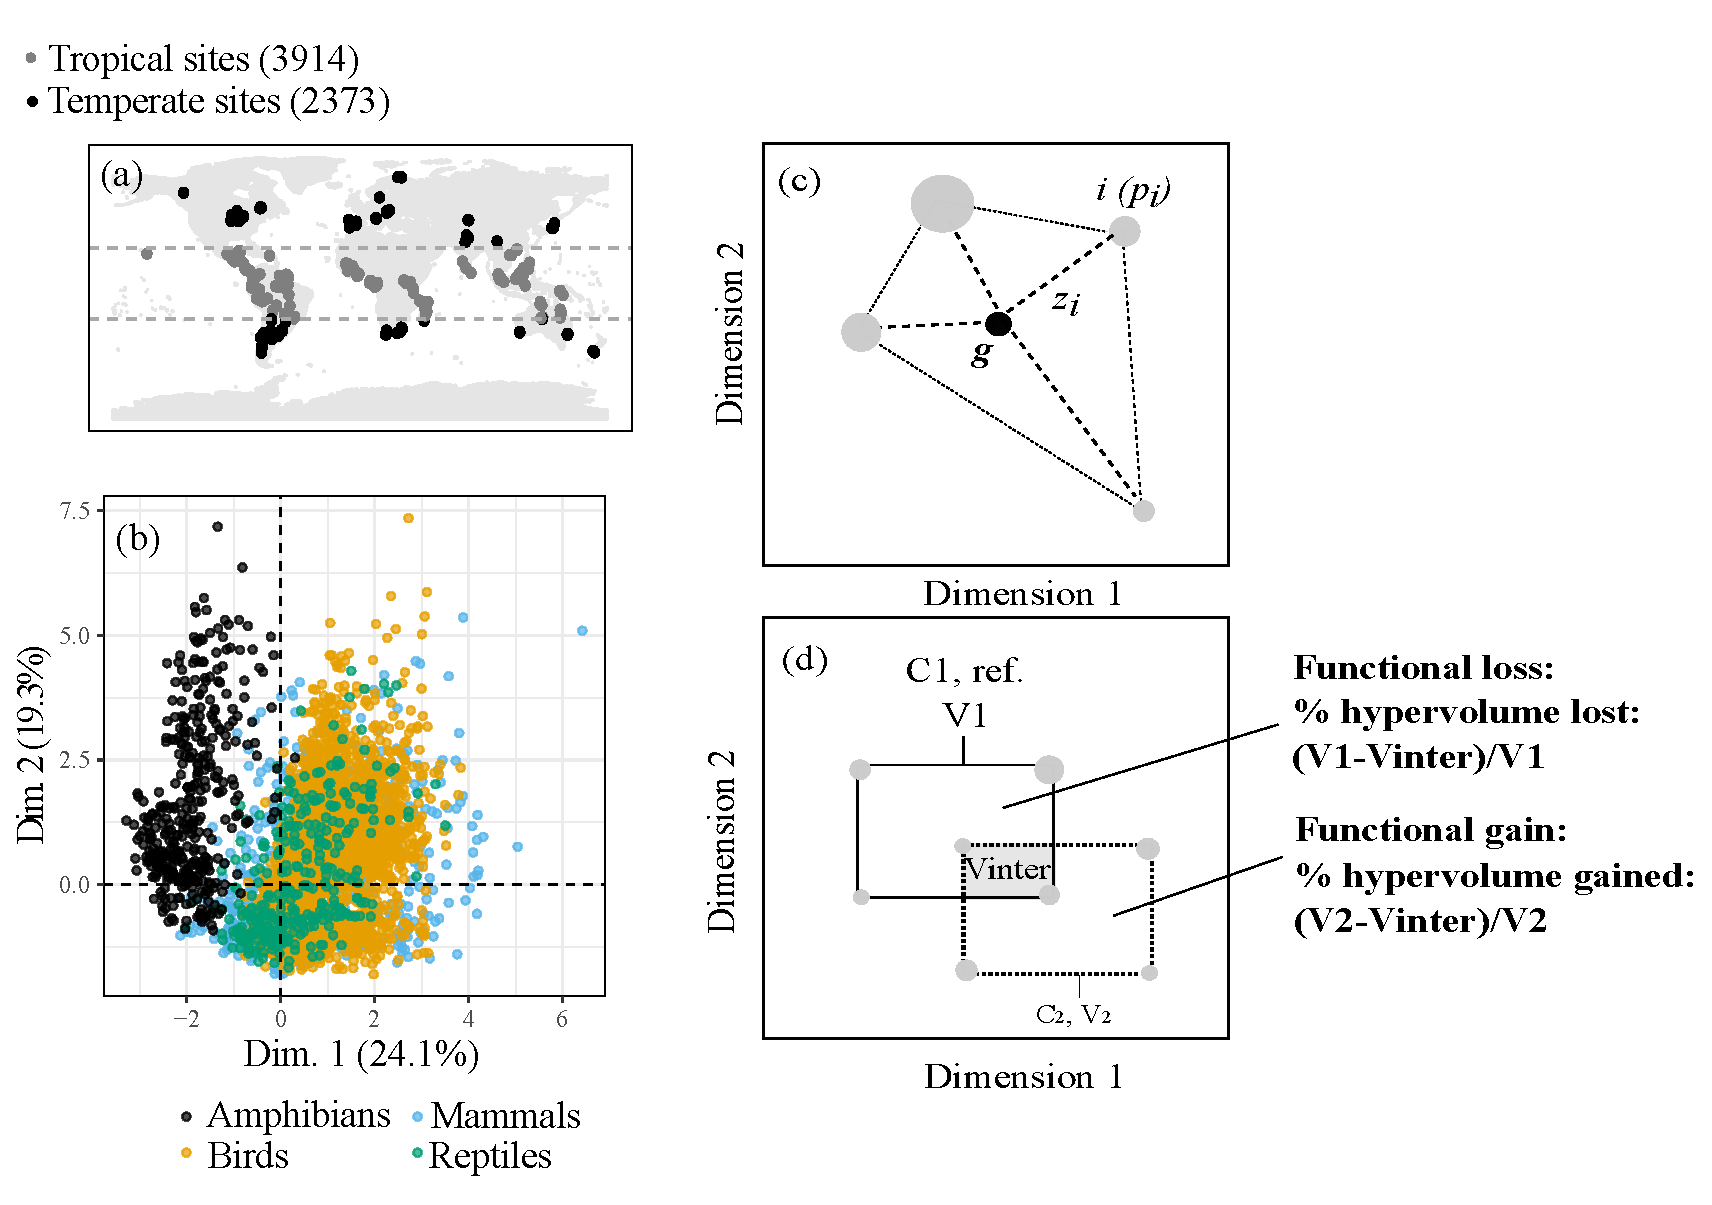
\includegraphics[scale=0.65]{figures/Chapter_FD/Figure1}
\caption[Overview of the study design and functional metrics.]{\textbf{Overview of the study design and functional metrics.} We used occurrence data for vertebrate species from the PREDICTS database (\citep{Hudson2014, Hudson2017}; 180 studies; 431,170 records; 4,339 species; 6,758 sampled sites). \textbf{(a)} shows the spatial distribution of sites we consider. We combine occurrence data with trait data compiled in Chapter 2 to calculate functional metrics. \textbf{(b)} is a representation of the trait data in two dimensions, plotted across PREDICTS vertebrates. Traits that contributed most to dimension 1 were lifespan (29\%) and litter/clutch size (22\%), while traits that contributed most to dimension 2 were habitat breadth (47\%) and use of artificial habitats (35\%). \textbf{(c)} and \textbf{(d)} present the conceptual framework for the calculation of the functional diversity metrics: local measures (c) and pairwise metrics (d). (c) Given a trait space, functional richness is calculated as the hypervolume occupied by the minimum convex hull encompassing all species \cite{Villeger2008}. Functional dispersion is calculated as the mean distance of the species to the centroid, \textbf{\textit{g}} \cite{Laliberte2010}. (d) We compute functional loss as the proportion of hypervolume lost from the reference assemblage, and we define functional gain as the proportion of hypervolume of the disturbed assemblage that was gained (proportion of novel trait space in the disturbed assemblage)}
\label{chart_taxcor}
\end{figure}



\section{Methods}

\subsection{Vertebrate assemblages}

I used vertebrate occurrence data from the PREDICTS database \citep{Hudson2014, Hudson2017}, a collection of studies that recorded species occurrence across multiple land uses and land-use intensities. In PREDICTS, each study contains several sites, which may be clustered into spatial blocks. Assemblage and land-use data are available at the site level: one site is characterised by a unique land use of given use intensity and provides occurrence data for a set of sampled taxa (and the same set of taxa is sought at all other sites within a study). Sites located between 23.5$^{\circ}$N and 23.5$^{\circ}$S of latitude were considered tropical, and otherwise temperate (Figure 1).

Land uses in PREDICTS were assigned to the following categories, based on the descriptions of the habitat given by the original collectors of the data: primary vegetation (considered to be the undisturbed reference); secondary vegetation; plantation forest; pasture; cropland; urban (considered human, or disturbed; Table S1;  \cite{Hudson2014, Hudson2017}). Secondary vegetation is further divided into three categories: mature, intermediate and young, depending on the stage of recovery of the vegetation. Use intensity is reported as minimal, light or intense, according to criteria that depended on the land-use type in question (e.g., crop diversity, degree of mechanisation and chemical inputs in cropland, or bushmeat harvesting and selective logging in primary vegetation; \cite{Hudson2014}). I excluded sites for which the land use could not be characterised or for which the stage of recovery of secondary vegetation was unclear. As the PREDICTS database is a collection of independent studies, the design of this study was not balanced: the sample size varied across land uses (Figures S1, S2), and across taxonomic groups (3103 species of birds; 531 mammals; 379 amphibians; 326 reptiles).

\subsection{Functional traits and diversity indices}

\subsection{Effects of land use and use intensity on FRic and FDis (Hypothesis 1)}

\subsection{Investigating functional under-dispersion (Hypothesis 2)}

\subsection{Functional loss and functional gain (Hypothesis 3)}

\section{Results}

\section{Discussion}
